\documentclass{beamer}

\usepackage[utf8]{inputenc}
\usepackage[italian]{babel}
\usepackage{graphicx}
\usepackage[font=tiny,labelfont=bf]{caption}

\usetheme{Madrid}

\graphicspath{ {./pics} }

\title[Serverless data pipeline]{Stateful serverless application for data pipeline processing}
\subtitle{SDCC project a.y. 2023/2024}
\author[Stefano Belli, 0350116]{Stefano Belli, matricola 0350116}
\institute[uniroma2]{Università degli Studi di Roma "Tor Vergata"}
\date{}

\newcommand{\dflvspace}{\vspace{10pt}}

\renewcommand{\footnotesize}{\tiny}

\setbeamertemplate{navigation symbols}{}

\begin{document}

\begin{frame}
    \titlepage
\end{frame}

\begin{frame}
    \frametitle{Agenda}
    \tableofcontents
\end{frame}

\section{Serverless SAGA pattern}
\begin{frame}
    \frametitle{Serverless SAGA pattern}

    Adattiamo il pattern SAGA al serverless computing\footnotemark: i \textbf{microservizi} diventano le \textbf{funzioni 
    serverless} e l'\textbf{orchestratore} è il coordinatore delle funzioni: in base al \textbf{valore di ritorno} 
    o a eventuali \textbf{errori} delle funzioni orchestrate, il coordinatore decide se proseguire con la 
    transazione o avviare un rollback.

    \footnotetext[1]{Tabby Ward (AWS), Rohan Mehta (AWS), and Rimpy Tewani (AWS) - "Implement the serverless saga pattern by using AWS Step Functions" - \url{https://docs.aws.amazon.com/prescriptive-guidance/latest/patterns/implement-the-serverless-saga-pattern-by-using-aws-step-functions.html}}
\end{frame}

\section{Servizi AWS utilizzati}
\begin{frame}
    \frametitle{Servizi AWS utilizzati}

    Per effettuare il deployment dell'applicazione è stato utilizzato AWS, e in particolare i seguenti servizi:

    \begin{itemize}
        \item \textbf{API Gateway}: configurazione dell'endpoint e route HTTP
        \item \textbf{Lambda}: per il serverless computing
        \item \textbf{Step Functions}: come coordinatore delle funzioni lambda
        \item \textbf{DynamoDB}: database serverless NoSQL di tipo chiave-valore
        \item \textbf{Secrets Manager}: storage crittografico gestito da AWS per memorizzare segreti
    \end{itemize}

\end{frame}

\section{Tabelle DynamoDB}
\begin{frame}
    \frametitle{Tabelle DynamoDB}

    \fontsize{9pt}{10pt}\selectfont

    Le tabelle necessarie a supportare la transazione sono 3:
    \begin{itemize}
        \item \texttt{validationStatus}: tabella di appoggio alla lambda \texttt{validate}
        \item \texttt{transformationStatus}: tabella di appoggio alla lambda \texttt{transform}
        \item \texttt{storeStatus}: tabella di appoggio alla lambda \texttt{store}
    \end{itemize}

    Tutte e 3 memorizzano la tupla ricevuta in input dalla lambda (\texttt{RawTuple}), l'ID della transazione 
    (\texttt{StoreRequestId}, uguale tra tutte le tabelle per la stessa transazione, \textit{partition key numerica}, assimilabile a una primary key di un RDBMS) e lo stato della transazione (\texttt{StatusReason})

    \dflvspace
    
    La tabella finale è \texttt{nycYellowTaxis} ed è consultabile dall'applicativo che effettua analisi sui
    dati (processamento vero e proprio). E' composta da item che hanno attributi distinti per tutti gli elementi
    separati dal carattere di separazione della CSV entry, e non più quindi una "\texttt{RawTuple}". Sono presenti in questa
    tabella \underline{solo} i dati processati \textbf{correttamente}. Viene mantenuto lo \texttt{StoreRequestId} (che rimane uguale a quello delle tabelle di appoggio, per la stessa transazione).
\end{frame}

\begin{frame}
    \frametitle{Tabelle DynamoDB: stato in base all'esito della transazione}

    \begin{exampleblock}{Transazione terminata con successo}
    Transazione (intesa come entry composta dagli attributi \texttt{StoreRequestId}, \texttt{RawTuple} e 
    \texttt{StatusReason}) presente in tutte le tabelle d'appoggio con \texttt{StatusReason} $= 0$ per ognuna di 
    esse.
    
    E' presente l'item corrispondente nella tabella finale \texttt{nycYellowTaxis}
    \end{exampleblock}

    \begin{alertblock}{Transazione fallita alla fase $i$-esima di preprocessing}
    L'entry corrispondente alla transazione è presente \underline{al più} nella tabella d'appoggio della fase $i$-
    esima fino a quella della prima fase, con \texttt{StatusReason} $\neq 0$ che ha stesso valore tra tutti i db di 
    appoggio.

    \textbf{NON} è presente l'item corrispondente nella tabella finale \texttt{nycYellowTaxis}
    \end{alertblock}
\end{frame}

\section{Lambda di autorizzazione}
\begin{frame}
    \frametitle{Lambda di autorizzazione}

    \fontsize{9pt}{10pt}\selectfont

    \begin{enumerate}

        \item La lambda \texttt{authorizer}, viene invocata dall'API gateway se viene agganciato a quest'ultimo 
        un'\textit{Authorizer}: gli viene passato un JSON object contenente un array che ha come chiave 
        \texttt{"identitySource"}, che ha in prima posizione la chiave di autenticazione inserita dal client HTTP 
        nell'header della richiesta - ovvero l'entry che ha come chiave \texttt{"Authorization"}.


        \item \texttt{authorizer} confronta quindi la chiave di autenticazione fornita dal client con quella impostata
        in fase di deployment e memorizzata in uno storage crittografico gestito da AWS Secrets Manager (chiedendone
        quindi la decrittazione).

        \item Ritornando un JSON object \texttt{\{ "isAuthorized": true \}} oppure 
    
        \texttt{\{ "isAuthorized": false \}}, 
        questa lambda permette all'API gateway di decidere se far "passare" o meno la richiesta.
        
    \end{enumerate}

    \begin{exampleblock}{Vantaggi}
    Si mitiga l'effetto di attacchi di tipo denial of service, che a causa del run delle lambda, diventano attacchi
    di tipo monetario, e proprio per quest'ultima ragione sarebbero solamente mitigati, e non risolti del tutto: comunque viene eseguita la lambda authorizer. Ma si elimina del tutto il problema di inserimenti non autorizzati
    \end{exampleblock}

    \fontsize{6pt}{10pt}\selectfont
    \centering
    \textit{(Il suo utilizzo è opzionale)}
    
\end{frame}

\section{Lambda di validazione}
\begin{frame}
    \frametitle{Lambda di validazione}

    \fontsize{10pt}{10pt}\selectfont

    Alla lambda di validazione, la prima nella catena di preprocessing, viene passata la tupla in "formato raw",
    ovvero una CSV entry (stringa): è la lambda che apre la transazione.

    \begin{enumerate}
        \item Calcola \texttt{StoreRequestId}, un ID univoco della transazione - a partire dalla tupla in input
        stessa (una "weak" hash function), il tempo UNIX al momento dell'invocazione della lambda e il valore 
        che restituisce un PRNG
        \item Inserisce nel proprio db di appoggio la tupla ricevuta in input, con l'ID di transazione e lo stato
        posto inizialmente a 0 (successo)
        \item Effettua validazione sui vari campi in base alle dizionario fornito dal sito della città di New York
        in merito dal dataset dei taxi gialli, controlla che le date siano corrette. Se la colonna non è ritenuta
        importante e il check fallisce, comunque "lascia correre" e la sostituisce con stringa vuota.
        \item Effettua validazione inter-colonna: constraint su più colonne.
        \begin{itemize}
            \item Check data "pickup" $<$ "dropoff"
            \item Check colonna somma di altre
        \end{itemize}
        \item Ritorna un JSON object che segnala la riuscita o meno dell'operazione, l'ID di transazione, la tupla 
        stessa (validata, trimmed + elim. campi) e il reason code (si vedano le lambda di flagging in seguito)
    \end{enumerate}
\end{frame}

\section{Lambda di trasformazione}
\begin{frame}
    \frametitle{Lambda di trasformazione}

    \fontsize{10pt}{10pt}\selectfont

    Riceve dalla lambda precedente, la tupla validata con l'ID univoco della transazione (è ovvio 
    che a questo punto, la parte di JSON object ricevuta in input rimanente che indica fallimenti in parte 
    precedente è:
    
    \texttt{\{\;"success":\;true,\;"reason":\;0,\;\dots\;\}}), quindi:

    \dflvspace

    \begin{enumerate}
        \item Inserisce l'entry nel suo db di appoggio composto da tupla ricevuta, ID univoco della transazione e 
        stato della transazione
        \item Effettua trasformazioni sulla tupla:
        \begin{itemize}
            \item Convertire un'enumerazione da intero a stringa secondo il dizionario del dataset
            \item Convertire da numero decimale a intero la colonna 4 (numeri erano espressi come $10.0$, $9.0$, $8.0$, \dots)
            \item Convertire data e ora in un altro formato
            \item Cambio carattere di separazione da ',' a '\textbackslash t' per la tupla (entry CSV)
        \end{itemize}

        \item Ritorna \texttt{\{\;"success":\;true,\;"reason":\;0,\;\dots\;\}} se la trasformazione è andata
        a buon fine, \texttt{\{\;"success":\;false,\;"reason":\;2,\;\dots\;\}} altrimenti.
        E' presente nel JSON object ritornato, anche la tupla trasformata e l'ID di transazione
    \end{enumerate}
\end{frame}

\section{Lambda di store}
\begin{frame}
    \frametitle{Lambda di store}

    \fontsize{10pt}{10pt}\selectfont

    L'ultima lambda da eseguire è quella che colleziona la tupla preprocessata nella tabella finale:

    Riceve lo stesso JSON object che riceveva \texttt{transform} da \texttt{validate}, solo con la tupla trasformata
    secondo le regole scritte per la trasformazione.
    
    \begin{enumerate}
        \item Inserisce la tupla trasformata ricevuta nella propria \underline{tabella di appoggio}, insieme, come 
        al solito, a ID univoco di transazione e stato della transazione.
        \begin{alertblock}{A che serve avere un'ulteriore tabella di appoggio?}
        Se dovesse fallire l'inserimento nella tabella finale, non viene persa la tupla raw trasformata!
        \end{alertblock}
        \item Costruisce l'entry per la tabella finale, separando opportunamente gli attributi (non è più una
        stringa di una riga CSV). Nell'entry della tabella finale viene mantenuto l'ID della transazione eseguita.
        \item Inserisce l'entry appena costruita nella \underline{tabella finale}
        \item Ritorna un JSON object \texttt{\{\;"success"\;:\;true\;\}}
    \end{enumerate}

    \fontsize{7pt}{10pt}\selectfont
    \textit{Vale la pena notare che la lambda di store non \textbf{fallisce} mai per \textbf{valore di ritorno} "unexpected", ma solamente per un \textbf{errore} (inserimento non riuscito in tabella)}
\end{frame}

\section{Lambda di flagging}
\begin{frame}
    \frametitle{Lambda di flagging}

    \fontsize{10pt}{10pt}\selectfont

    Le lambda di flagging \texttt{flagValidateFailed}, \texttt{flagTransformFailed} e \texttt{flagStoreFailed}
    condividono lo stesso identico codice: è stato realizzato un modulo Go \texttt{flagPhaseFailed} che generalizza
    queste lambda che modificano l'entry nella propria tabella di competenza al verificarsi di un fallimento
    di transazione.

    \dflvspace

    Il modulo, in base all'input fornito dalla state machine:
    \begin{itemize}
        \item \textbf{E' già in grado di recuperare il codice d'errore reason} - la transazione è fallita perchè
        la lambda corrispondente a una certa fase ha \textbf{ritornato} un JSON object diverso da quanto ci si 
        sarebbe aspettati (il codice d'errore è indicato direttamente dalla lambda fallita)
        \item \textbf{Deve dedurre il codice d'errore reason} - lo fa dalle informazioni sull'\textbf{errore}, che 
        ha causato fallimento della lambda corrispondente a una certa fase, incluse \underline{dalla state machine}
        nell'input alla lambda di flagging
    \end{itemize}

    \dflvspace

    Una volta dedotto, viene aggiornata l'entry corrispondente alla tabella di appoggio (in base alla partition key 
    \texttt{StoreRequestId}) di competenza, con il codice di stato corrispondente alla fase di preprocessing che ha 
    causato fallimento
    
\end{frame}

\section{State machine}
\begin{frame}
    \frametitle{State machine}

    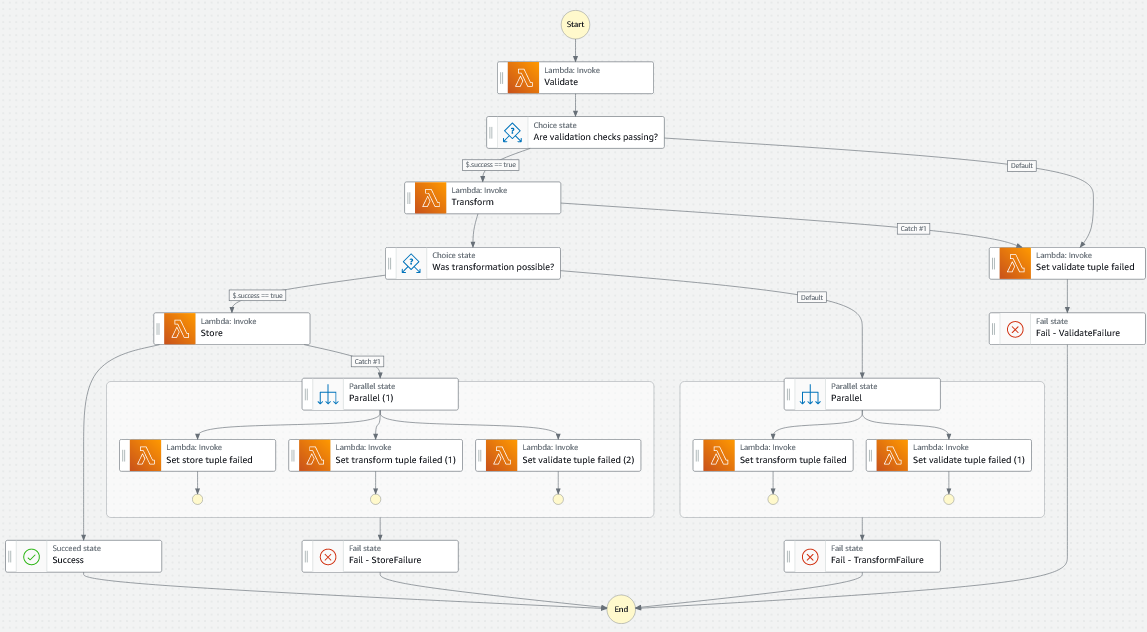
\includegraphics[width=12cm, height=7cm]{whole-sfn}
\end{frame}

\begin{frame}
    \frametitle{}
    
    \fontsize{30pt}{10pt}\selectfont
    \centering
    \textbf{Grazie per l'attenzione!}
    
\end{frame}

\end{document}